\documentclass[aspectratio=169]{beamer}

\usetheme{Madrid}
\usecolortheme{default}

\usepackage{amsmath}
\usepackage{booktabs}
\usepackage[T1]{fontenc}
\usepackage{graphicx}
\usepackage[utf8]{inputenc}
\usepackage{listings}
\usepackage{lmodern}
\usepackage{xcolor}
\graphicspath{{./}{public/presentation/}{./public/presentation/}}

\definecolor{bgTop}{HTML}{09111D}
\definecolor{bgBottom}{HTML}{050A12}
\definecolor{panelBg}{HTML}{0A111E}
\definecolor{panelSoft}{HTML}{0E1625}
\definecolor{textPrimary}{HTML}{E4EDF7}
\definecolor{textMuted}{HTML}{BED0E2}
\definecolor{textFaint}{HTML}{8FA6BF}
\definecolor{accentMint}{HTML}{82F0D2}
\definecolor{accentAmber}{HTML}{F4B35F}
\definecolor{accentSlate}{HTML}{6C7F93}
\definecolor{lineColor}{HTML}{304358}

\title{Buffon's Needle}
\subtitle{Randomness, Geometry, and an Estimate of $\pi$}
\author[Group 18]{Enci XU 20719529, Xu WANG 20719627, Zekai FU 20719631, Zhe CAO 20721357, Kangjun XU 20719527, Zihan ZHU 20719640}
\date{April 3, 2026}

\setbeamercolor{background canvas}{bg=bgBottom}
\setbeamercolor{normal text}{fg=textPrimary,bg=bgBottom}
\setbeamercolor{frametitle}{fg=accentMint,bg=panelBg}
\setbeamercolor{title}{fg=textPrimary}
\setbeamercolor{subtitle}{fg=textMuted}
\setbeamercolor{author}{fg=textMuted}
\setbeamercolor{institute}{fg=textFaint}
\setbeamercolor{date}{fg=textFaint}
\setbeamercolor{structure}{fg=accentMint}
\setbeamercolor{section in toc}{fg=textPrimary}
\setbeamercolor{subsection in toc}{fg=textMuted}
\setbeamercolor{palette primary}{fg=textPrimary,bg=panelBg}
\setbeamercolor{palette secondary}{fg=textMuted,bg=panelSoft}
\setbeamercolor{palette tertiary}{fg=textPrimary,bg=panelBg}
\setbeamercolor{palette quaternary}{fg=textMuted,bg=panelSoft}
\setbeamercolor{block title}{fg=bgBottom,bg=accentMint}
\setbeamercolor{block body}{fg=textPrimary,bg=panelBg}
\setbeamercolor{block title alerted}{fg=bgBottom,bg=accentAmber}
\setbeamercolor{block body alerted}{fg=textPrimary,bg=panelBg}
\setbeamercolor{block title example}{fg=bgBottom,bg=accentSlate}
\setbeamercolor{block body example}{fg=textPrimary,bg=panelBg}
\setbeamercolor{item}{fg=accentMint}
\setbeamercolor{subitem}{fg=accentMint}
\setbeamercolor{enumerate item}{fg=accentAmber}
\setbeamercolor{caption name}{fg=accentMint}
\setbeamercolor{footline}{fg=textFaint,bg=panelBg}
\setbeamercolor{headline}{fg=textFaint,bg=panelBg}
\setbeamercolor{titlelike}{fg=textPrimary}

\definecolor{codebg}{HTML}{0E1625}
\definecolor{codekw}{HTML}{82F0D2}
\definecolor{codestr}{HTML}{F4B35F}
\definecolor{codecomment}{HTML}{8FA6BF}

\lstset{
  basicstyle=\ttfamily\small,
  backgroundcolor=\color{codebg},
  keywordstyle=\color{codekw}\bfseries,
  stringstyle=\color{codestr},
  commentstyle=\color{codecomment},
  identifierstyle=\color{textPrimary},
  numberstyle=\color{textFaint},
  showstringspaces=false,
  breaklines=true,
  frame=single,
  rulecolor=\color{lineColor}
}

\setbeamertemplate{navigation symbols}{}
\addtobeamertemplate{headline}{}{%
  \hfill
  \raisebox{-0.85cm}[0pt][0pt]{
\includegraphics[height=0.6cm]{nottingham-school-logo-white.png}}
  \hspace{0.35cm}
}

\begin{document}

\begin{frame}
  \titlepage
\end{frame}

\begin{frame}{Outline}
  \tableofcontents
\end{frame}

\section{Why This Problem}

\begin{frame}{A Simple Puzzle with a Big Idea}
  \begin{columns}[T]
    \begin{column}{0.56\textwidth}
      \begin{itemize}
        \item Buffon posed the needle problem in the 18th century.
        \item A random experiment can reveal a precise constant: $\pi$.
        \item It is an early example of geometric probability.
        \item It also anticipates the Monte Carlo idea: estimate by repeated random trials.
      \end{itemize}
    \end{column}
    \begin{column}{0.4\textwidth}
      \begin{block}{Core question}
        If we drop a needle onto equally spaced parallel lines, how often does it cross a line?
      \end{block}
    \end{column}
  \end{columns}
\end{frame}

\section{Geometry to Formula}

\begin{frame}{Setup and Crossing Rule}
  \begin{columns}[T]
    \begin{column}{0.48\textwidth}
      \begin{block}{Experiment setup}
        \begin{itemize}
          \item Line spacing: $d$
          \item Needle length: $l \le d$
          \item Angle to the lines: $\theta \in [0,\pi]$
          \item Midpoint distance to the nearest line: $x \in [0,d/2]$
        \end{itemize}
      \end{block}
    \end{column}
    \begin{column}{0.48\textwidth}
      \begin{alertblock}{Crossing region}
        The needle crosses a line when
        \[
          x \le \frac{l}{2}\sin\theta.
        \]
        So for each fixed $\theta$, the allowed values of $x$ are
        \[
          0 \le x \le \frac{l}{2}\sin\theta.
        \]
      \end{alertblock}
    \end{column}
  \end{columns}
\end{frame}

\begin{frame}{Theory: Sample Space and Favourable Region}
  \begin{columns}[T]
    \begin{column}{0.5\textwidth}
      \begin{block}{By symmetry}
        Instead of using every angle in $[0,\pi]$, we can work on the smaller sample space
        \[
          x \in \left[0,\frac{d}{2}\right],
          \qquad
          \theta \in \left[0,\frac{\pi}{2}\right].
        \]
        The total area is therefore
        \[
          A_{\text{total}} = \frac{d}{2}\cdot\frac{\pi}{2} = \frac{\pi d}{4}.
        \]
      \end{block}
    \end{column}
    \begin{column}{0.46\textwidth}
      \begin{exampleblock}{Favourable area}
        \[
          A_{\text{fav}}
          =
          \int_0^{\pi/2}\int_0^{(l/2)\sin\theta} dx\,d\theta.
        \]
      \end{exampleblock}
    \end{column}
  \end{columns}
\end{frame}

\begin{frame}{Theory: Why \texorpdfstring{$\pi$}{pi} Appears}
  \begin{columns}[T]
    \begin{column}{0.52\textwidth}
      \begin{block}{Evaluate the integral}
        \[
          A_{\text{fav}}
          =
          \int_0^{\pi/2}\frac{l}{2}\sin\theta\,d\theta
          =
          \frac{l}{2}.
        \]
        Hence
        \[
          P(\text{cross})
          =
          \frac{A_{\text{fav}}}{A_{\text{total}}}
          =
          \frac{l/2}{\pi d/4}
          =
          \frac{2l}{\pi d}.
        \]
      \end{block}
    \end{column}
    \begin{column}{0.44\textwidth}
      \begin{alertblock}{Special case in our demo}
        When $l=d=1$,
        \[
          P(\text{cross}) = \frac{2}{\pi} \approx 0.63662.
        \]
      \end{alertblock}
      \begin{exampleblock}{Estimator}
        After $N$ throws and $C$ crossings,
        \[
          \hat{P} = \frac{C}{N},
          \qquad
          \hat{\pi} \approx \frac{2N}{C}.
        \]
      \end{exampleblock}
    \end{column}
  \end{columns}
\end{frame}

\section{Simulation}

\begin{frame}[fragile]{Simulation Logic and One Sample Run}
  \begin{columns}[T]
    \begin{column}{0.5\textwidth}
      \begin{lstlisting}[language=Python]
repeat N times:
    sample theta in [0, pi]
    sample x in [0, d/2]
    if x <= (l/2) * sin(theta):
        C <- C + 1

if l = d = 1:
    pi_hat <- 2*N / C
      \end{lstlisting}
      \vspace{0.15em}
      \centering
      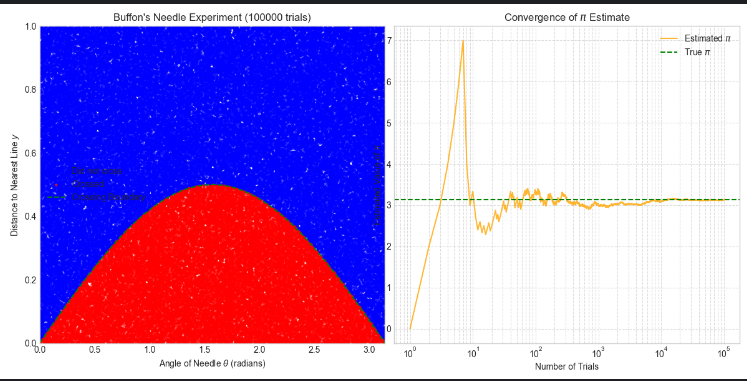
\includegraphics[width=0.78\linewidth]{python-figure.png}
    \end{column}
    \begin{column}{0.46\textwidth}
      \begin{table}
        \centering
        \small
        \begin{tabular}{rcc}
          \toprule
          $N$ & $C$ & $\hat{\pi}$ \\
          \midrule
          100 & 60 & 3.3333 \\
          1,000 & 628 & 3.1847 \\
          10,000 & 6,401 & 3.1245 \\
          100,000 & 63,753 & 3.1371 \\
          \bottomrule
        \end{tabular}
      \end{table}
      \begin{exampleblock}{Take-away}
        The estimate fluctuates at first, then settles near $\pi$ as the number of trials grows.
      \end{exampleblock}
    \end{column}
  \end{columns}
\end{frame}

\section{Extensions and Uses}

\begin{frame}{Beyond a Straight Needle -- Moser's Curved Needle}
  \begin{columns}[T]
    \begin{column}{0.48\textwidth}
      \begin{block}{Q}
        What happens if we replace the straight needle with a curve?
      \end{block}

      \begin{alertblock}{A}
        For a curved needle, the expected number of intersections depends on the total length rather than the exact shape.
      \end{alertblock}
    \end{column}
    \begin{column}{0.48\textwidth}
      \begin{exampleblock}{Link}
        A sufficiently regular curve can be approximated by many tiny straight segments.
      \end{exampleblock}

      \begin{block}{Main idea}
        Bending changes the geometry locally, but the expectation is governed by total length.
      \end{block}
    \end{column}
  \end{columns}
\end{frame}

\section{Demo}

\begin{frame}{Live Web Demo}
  \small
  \begin{columns}[T]
    \begin{column}{0.6\textwidth}
      \begin{block}{Open the demo}
        \href{https://buffons-needle.byron.wang/}{\textcolor{accentMint}{\texttt{https://buffons-needle.byron.wang/}}}
      \end{block}
      {\scriptsize \textcolor{textMuted}{Open-sourced on GitHub under the MIT License.  Copyright belongs to our group.}}
      \vspace{0.2em}
      \begin{itemize}
        \item Drop 1 or 100 needles, or switch to auto-run.
        \item Compare $C/N$ with the theoretical value $2/\pi$.
        \item Watch the estimate $\hat{\pi}$ stabilise in real time.
      \end{itemize}

      \vspace{0.15em}

      \begin{alertblock}{Closing idea}
        A simple random rule can recover a famous constant, and the web demo shows that convergence live.
      \end{alertblock}
    \end{column}
    \begin{column}{0.28\textwidth}
      \centering
      \setlength{\fboxsep}{4pt}
      \fcolorbox{accentMint}{white}{
\includegraphics[width=0.72\linewidth]{buffons-needle-demo-qr.png}}

      \vspace{0.35em}

      {\small \textcolor{textMuted}{Scan to open the demo on your phone}}
    \end{column}
  \end{columns}
\end{frame}

\begin{frame}
  \centering
  \Huge Thank You
\end{frame}

\end{document}
